%!TEX root = ../dokumentation.tex
\chapter{Continuous Integration}\label{ch:continuous-integration}
Als CI wurde am Anfang AWS CodePipeline verwendet. Dies bot eine einfach Einbindung zwischen Github und AWS Elastikbeanstalk. Sobald Der Master des Github Repositories einen neuen Push erhalten hat, wurde automatisch der neue Code auf den Server geladen. Jedoch als später Tests zum Projekt hinzugefügt wurden, wollten wir, dass automatisch die Tests vor dem Deploy ausgeführt werden. Dazu wäre AWS CodeBuild eine Möglichkeit gewesen. Doch persönlich wurde bereits mit Travis-CI gearbeitet, was eine kostenlose und einfach implementierte Version darstellt. Für Travis CI muss man nur dem Programm Berechtigungen für das Github Repository geben, sowie eine .travis.yml Datei im Root des Repositories vorhanden sein. In dieser yml-Datei spezifiziert man Befehle die in einer bestimmten Reihenfolge ablaufen. Außerdem wurde AWS CodePipeline nicht mehr benötigt, da Travis CI eine eigene kostenlose Deploy Möglichkeit bereitstellt.
Dadurch wird nach jedem Push auf den Master des Github Repositories bei Travis CI eine virtuelle Umgebung aufgebaut die die definierten Befehle ausführt. Schlägt ein Build fehl wird es gestoppt. Den Status des Builds erkennt man an der build Badge in der ReadMe Datei. Sehen Sie hier den letzten Build des Projektes: https://travis-ci.com/github/Drinkler/Planning-Poker.
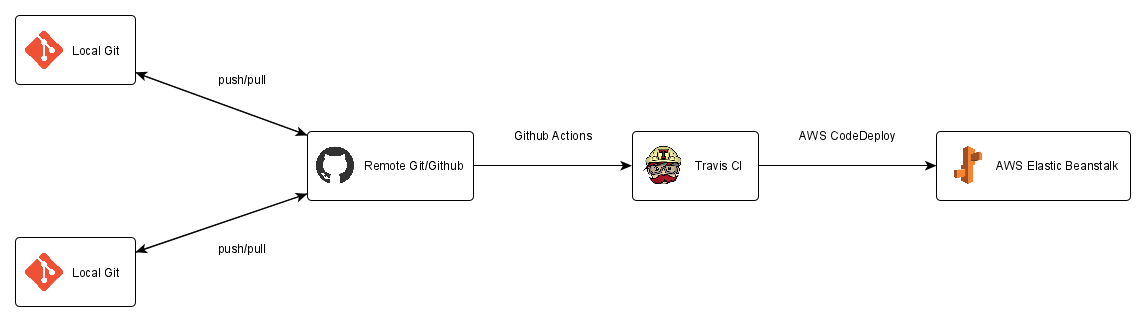
\includegraphics[width=\textwidth]{images/continuous_integration.png}

travis ci - aws codedeploy -> encrypted keys
github app / actions